\chapter{Week 7: 3\textsuperscript{rd} - 9\textsuperscript{th} Nov }

\tocless\section{Objectives}



\begin{itemize*}
	\item Read up on methods to remove bias from sensors.
	\item Analysis and remove offset/mean from accelerometer and gyroscope.
	\item Come up with a method to find the {\bf R} matrix of the system.
\end{itemize*}


\tocless\section{Accelerometer Bias }
Due to the fact of the large bias on the accelerometer a method had to be found in order to reduce it, a better model made to be found or the Kalman filter had to be remodelled. The method agreed approved to deal with this problem and hopefully the correct one is the methods discussed in the following papers
\cite{acclerometer_bais,Accelrometer_bias}. Upon using the sensors there were sensor bias error, however, the sensors can read something different that the required (ideal) at a given location due to many factors including mechanical tolerances in the component parts.


The way to measure and remove bias error from the accelerometer is to do the following:- 

\begin{enumerate}
	\item Place the sensor module on an approximately horizontal surface (table top, granite flat, etc.).
	\item Rotate the sensor module $90^o$ to each of the positions shown in
	      Figure
	\item Read the outputs on each axis in each of the six positions.
	\item Calculate the sensitivities (where the first subscript is the sensor, the second subscript is the position):
	      \begin{equation}
		      S_{xx} = \frac{(a_{x2} - a_{x4})}{2};~~S_{yy} = \frac{(a_{y1} - a_{y3})}{2};~~S_{zz} = \frac{(a_{z5} - a_{z6})}{2};
	      \end{equation}
	      
	\item
	      Calculate the sensor module biases:
	      
	      \begin{multline}
		      B_x^{0g} = \left(\frac{a_{x1}+a_{x3}+a_{x5}+a_{x6}}{4}\right);~~ B_y^{0g} = \left(\frac{a_{x2}+a_{x4}+a_{x5}+a_{x6}}{4}\right);\\B_z^{0g} = \left(\frac{a_{x1}+a_{x2}+a_{x3}+a_{x4}}{4}\right);
	      \end{multline}
	      
	\item Save $B_x^{0g}, ~ B_y^{0g},~B_z^{0g},~S_{xx},~S_{yy},~\mathrm{and}~S_{zz}$ local and use these values in all subsequent calculations of the acceleration to get the correct outputs.
\end{enumerate}

\begin{figure}[h]
	\centering
	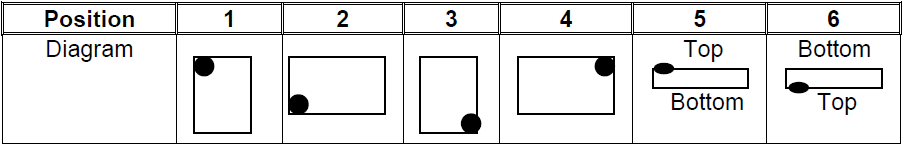
\includegraphics[width =0.6 \paperwidth]{\DocRoot/images/Bias}
	\caption{Position in which one has to measure the bias for calibration}
	\label{Fig: Position to measure the bias}
\end{figure}

\tocless\section{Formula to measure angle}
\tocless\subsection{Measuring Tilt Angle using One Axis}
Accelerometers measure acceleration. That is acceleration due to movement and also acceleration due to gravity. If you want to measure tilt in both $x$ and $y$ axis with a 2-axis accelerometer then you can simply use $\sin x$ where $x$ is the output from one axis of the accelerometer. Remember that beyond +45 and -45 degrees the accuracy will diminish

\tocless\subsection{Measuring Tilt Angle using Three Axis}
For accurate measurements of tilt in both the $x ~\mathrm{\&}~ y $ planes the following formulas have to be used\footnote{See \url{http://www.hobbytronics.co.uk/accelerometer-info} for more details}
.

\begin{align}
	\begin{split}
		\gls{pitch} &= \arctan\left(\frac{\gls{ax}}{\sqrt{\gls{ay}^2 + \gls{az}^2}}\right)\\
		\gls{roll} &= \arctan\left(\frac{\gls{ay}}{\sqrt{\gls{ax}^2 + \gls{az}^2}}\right)
	\end{split}
\end{align}
